%-------------------------------------------------------------------------------
% APPENDICES 
%-------------------------------------------------------------------------------

\begin{appendices}

\section{Implementation of Boundary Conditions in Julia}

\begin{jllisting}[caption={Boundary construction function for the matrix
  $\Psi$, below the inplace and out of place versions of this function
  \vspace{3pt}}]
function constructBC!(Ψ, p::CavityStruct)
    @unpack m, D1, a11, a12, a21, a22 = p.params 
    @unpack bcleft, bcright, bctop, bcbottom = p.params
    @unpack h1, h2, k1, k2 = p.cache

    @inbounds @views Ψ1 = Ψ[3:(m - 1), 3:(m - 1)]
    @inbounds @views Ψ2 = Ψ[3:(m - 1), 2:m]'
    @inbounds @views Dcs = D1[1, 3:(m - 1)]
    @inbounds @views Dce = D1[m + 1, 3:(m - 1)]

    mul!(h1, Ψ1, Dcs)
    mul!(h2, Ψ1, Dce)

    @inbounds @views @. Ψ[3:(m - 1), 2] = a11 * (bctop[3:(m - 1)] - h1) +
                                          a12 * (bcbottom[3:(m - 1)] - h2)
    @inbounds @views @. Ψ[3:(m - 1), m] = a21 * (bctop[3:(m - 1)] - h1) +
                                          a22 * (bcbottom[3:(m - 1)] - h2)

    mul!(k1, Ψ2, Dcs)
    mul!(k2, Ψ2, Dce)

    @inbounds @views @. Ψ[2, 2:m] = a11 * (bcleft[2:m] - k1) +
                                    a12 * (bcright[2:m] - k2)
    @inbounds @views @. Ψ[m, 2:m] = a21 * (bcleft[2:m] - k1) + 
                                    a22 * (bcright[2:m] - k2)

    return nothing
end

function constructBC(u, p::CavityStruct)
    @unpack m = p.params

    Ψ = zeros(m + 1, m + 1)
    @inbounds @views Ψ[3:(m - 1), 3:(m - 1)][:] .= u

    constructBC!(Ψ, p)

    return Ψ
end
\end{jllisting}

The code snippet shows how the outer rows and columns are computed to
incorporate the boundary conditions. \jlinl{a11}, \jlinl{a12}, \jlinl{a21} and
\jlinl{a22} are the pre-computed elements of the inverse of the matrix $A$ in
equation \eqref{eq:mat1}. As the domain is square ($(m+1) \times (m+1)$), this
matrix is the same for both spatial directions. The variables with a \jlinl{bc}
in front correspond the prescribed values for the grid points at the boundary.

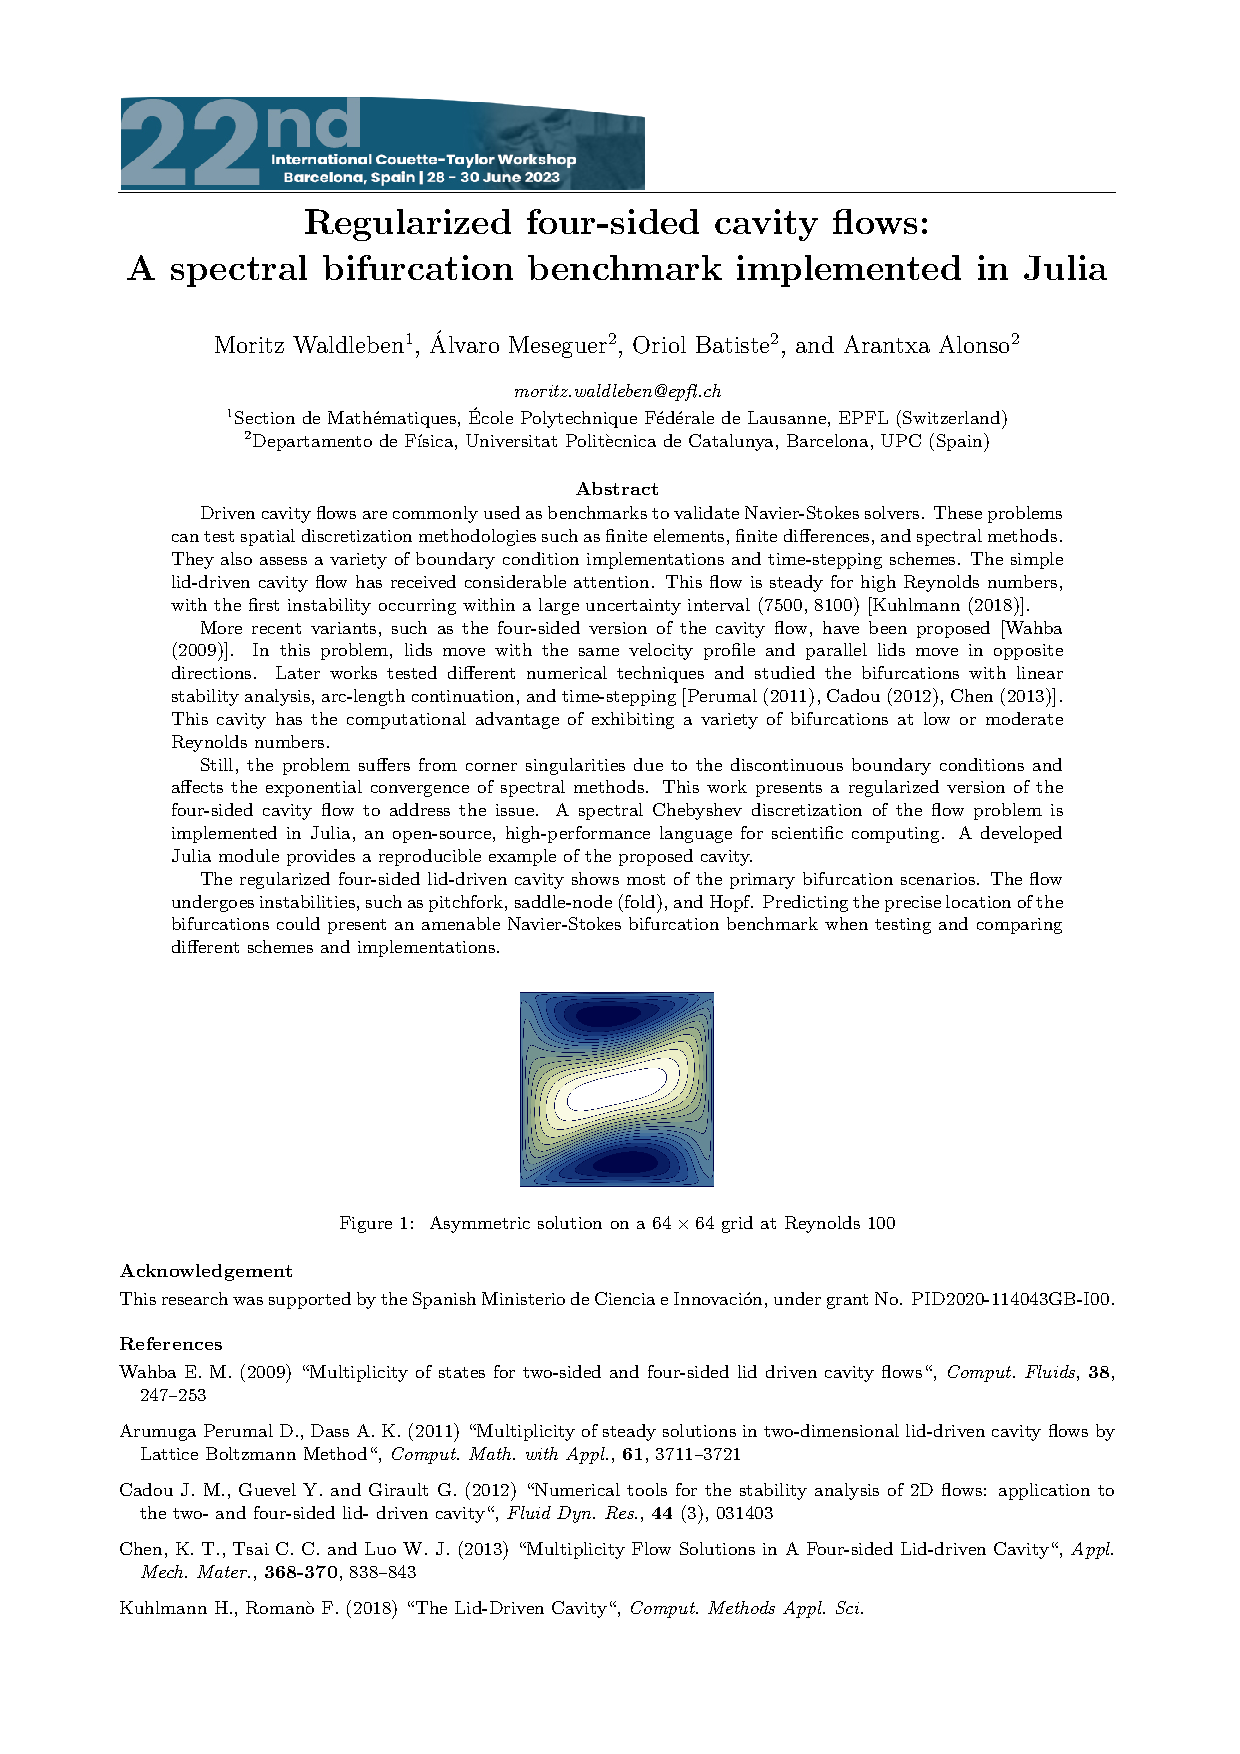
\includepdf[
  scale=0.8,
  offset=75 -75,
  pagecommand=\section{Abstract Conference Presentation at ICTW 2023}
  ]{figs/ictw23_abstract.pdf}

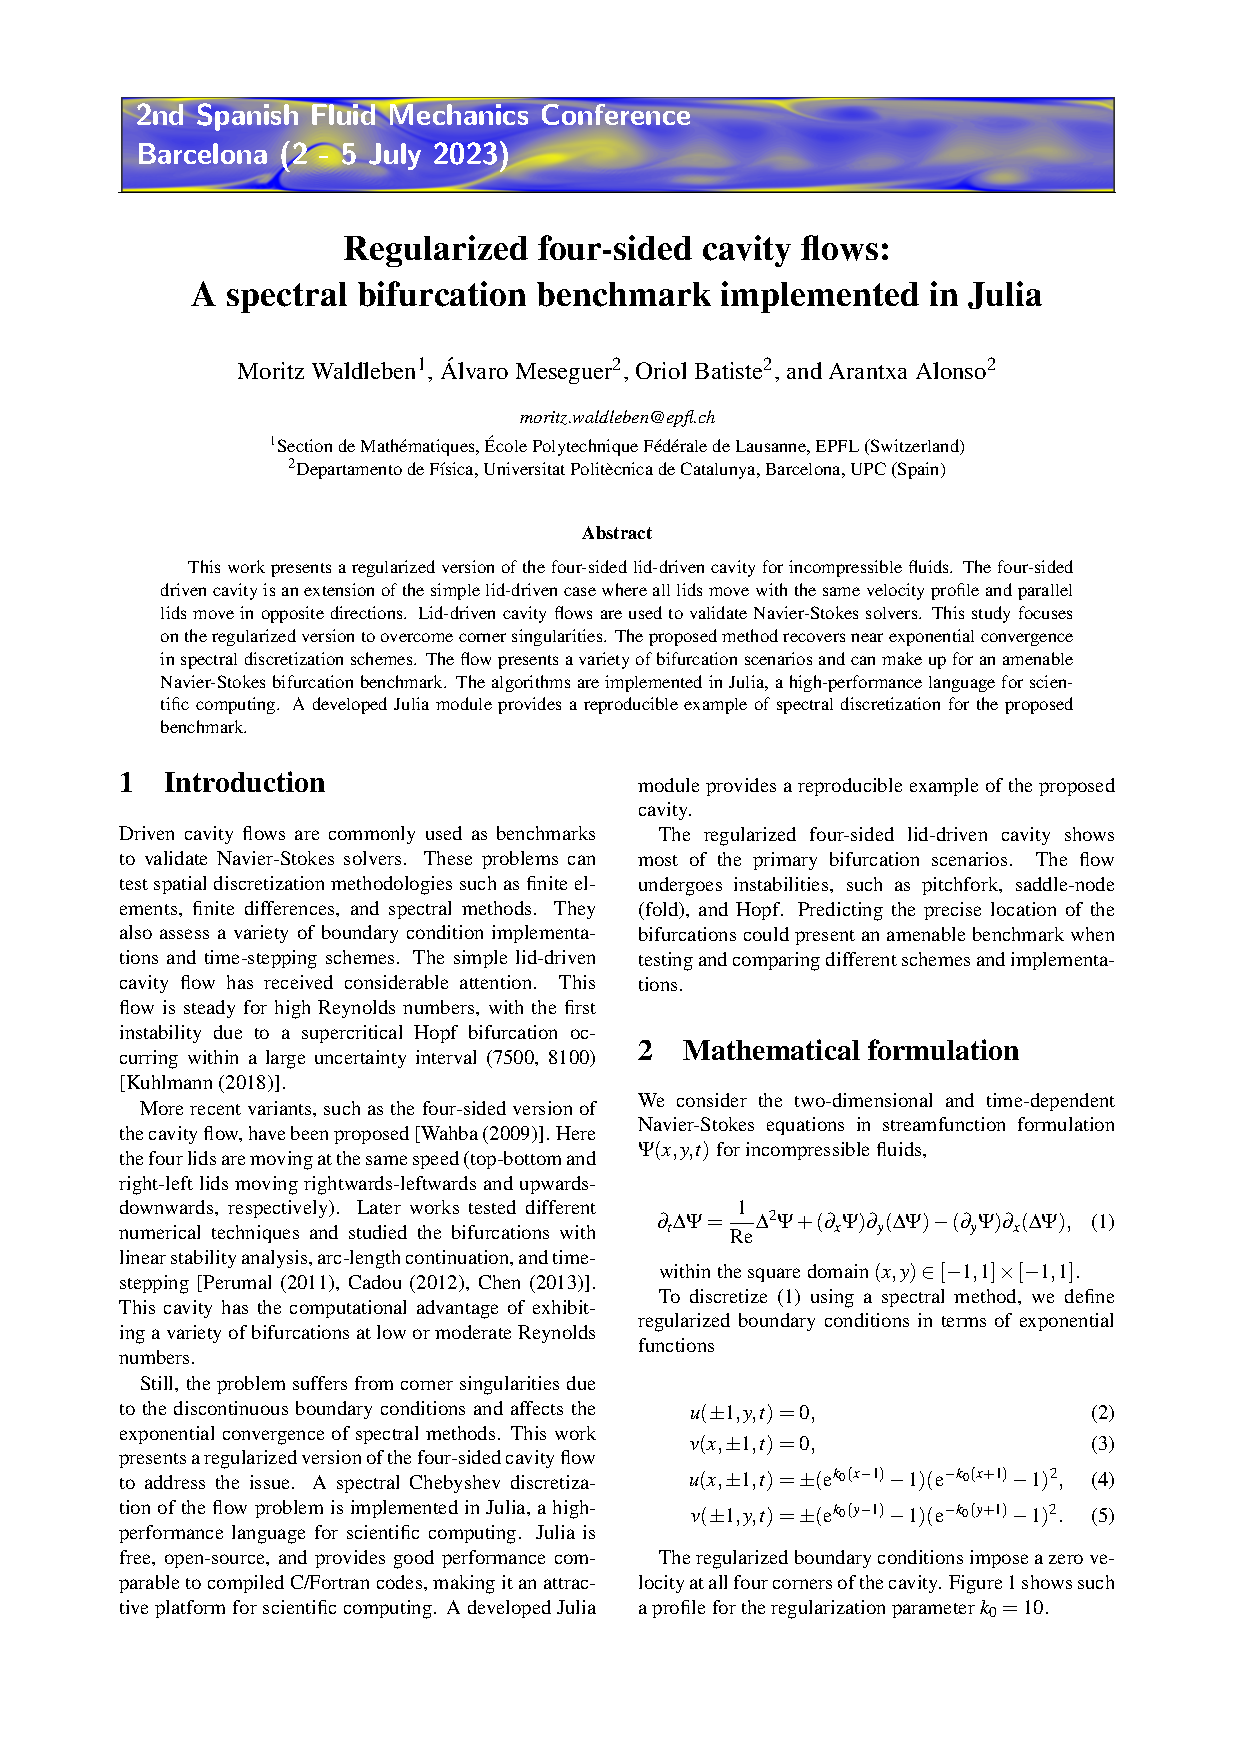
\includepdf[
  scale=0.8,
  pages=1,
  offset=75 -75,
  pagecommand=\section{Abstract Conference Presentation at SFMC 2023}
]{figs/sfmc23_abstract.pdf}
\includepdf[
  scale=0.8,
  pages=2,
  offset=75 -75,
  pagecommand={},
  trim=0 2cm 0 2cm,
  clip
]{figs/sfmc23_abstract.pdf}

\end{appendices}
